\documentclass[11pt]{article}

% Use the [review] option for anonymized submission (adds line numbers).
% Switch to \usepackage{acl} (no option) for the camera-ready version.
\usepackage[review]{acl}

\usepackage{times}
\usepackage{latexsym}
\usepackage[T1]{fontenc}
\usepackage[utf8]{inputenc}
\usepackage{microtype}

\usepackage{graphicx}
\usepackage{subcaption}
\usepackage{booktabs}
\usepackage{amsmath,amssymb}
\usepackage{multirow}
\usepackage{float}

% Keep review line numbers out of the text on every page.
% Stock acl.sty loads lineno with [switch], which flips all numbers to one
% side by page parity; on even pages they land in the gutter over the text.
% Place them by column instead: left column -> left margin, right column ->
% right margin (outer margins), consistent on every page.
\makeatletter
\AtBeginDocument{%
  \@ifpackageloaded{lineno}{%
    \def\makeLineNumber{%
      \if@firstcolumn\makeLineNumberLeft\else\makeLineNumberRight\fi}%
  }{}%
}
\makeatother

\title{Nested Sycophancy:\\Probes Find Asymmetric Mechanisms Across Three LLM Architectures,\\But Static Steering Fails}

\author{Anonymous ACL submission}

\begin{document}
\maketitle

\begin{abstract}
Sycophancy---agreeing with users at the expense of honesty---has a nested internal geometry: it is readable by linear probes but not writable by static linear steering.
We train linear probes on residual stream activations stratified by token-level entropy across three reasoning models: Qwen3-14B (dense), gpt-oss-20b (MoE, $32 \times 4$ routing), and Qwen3-30B-A3B (MoE, $128 \times 8$ routing).
Probes trained on uncertain examples transfer to confident examples near-losslessly ($\Delta\mathrm{AUROC} \leq 0.03$), while confident probes fail on uncertain data ($\Delta \geq 0.25$).
This indicates that the uncertain-sycophancy direction $\mathbf{w}_{\text{unc}}$ captures a shared drift component present in both regimes, whereas confident sycophancy adds a nearly orthogonal override direction $\mathbf{v}_{\text{override}}$ ($\cos(\mathbf{w}_{\text{conf}}, \mathbf{w}_{\text{unc}}) \approx 0.06$--$0.10$).
Subspace inclusion analysis confirms the asymmetry with high significance in two of the three models ($p < 0.001$), with suggestive but non-significant trends in gpt-oss-20b ($p = 0.096$).
Router-level analysis in both MoE models shows that confident and uncertain inputs are processed by the same fixed expert subsets (``standing committees'', Jaccard $\geq 0.86$), localizing the nested geometry to within-expert computation rather than routing.
Finally, static linear steering along either direction yields $\leq 2$ pp sycophancy reduction before generation collapses---an empirical instance of representational independence violation: orthogonal probe directions are not causally independent under intervention.
These results motivate regime-aware, on-manifold interventions, for which the $(\mathbf{w}_{\text{unc}}, \mathbf{v}_{\text{override}})$ basis provides the diagnostic components.
Code and data are publicly released.
\end{abstract}

% ============================================================================
\section{Introduction}
\label{sec:intro}

Sycophancy, the tendency of language models to agree with users rather than provide honest answers, is one of the most persistent failure modes of RLHF-trained systems \citep{sharma2024towards}.\footnote{Code: \url{https://anonymous.4open.science/r/sycophancy-uncertainty-E898/}; data: \url{https://huggingface.co/datasets/anonymous-author-1/nested-sycophancy}.}
The problem is exacerbated by epistemic uncertainty: when models lack confidence in their own knowledge, they are more susceptible to social pressure \citep{zhong2025investigating}.
Recent work has made important progress in decomposing sycophancy mechanistically.
\citet{jiang2025sycophancy} demonstrate causal separation of distinct sycophantic behaviors (flattery vs.\ agreement) onto orthogonal vectors.
\citet{mirtaheri2026motivated} show that motivated reasoning is encoded in the residual stream before chain-of-thought generation begins.

Our work takes the next step: from demonstrating that \emph{multiple} sycophancy mechanisms exist to characterizing their \emph{topological relationship}.
Within factual agreement, we discover that ``confident sycophancy'' (the model knows the truth but capitulates) and ``uncertain sycophancy'' (the model defers under epistemic deficit) are \emph{nested}: the discriminant subspace of uncertain sycophancy is contained within that of confident sycophancy.
Uncertain sycophancy ($\mathbf{w}_{\text{unc}}$) acts as a shared drift toward the persona-aligned answer; confident sycophancy adds an orthogonal truth-override ($\mathbf{v}_{\text{override}}$).
In MoE models, this geometry is computed within \emph{standing committees}, fixed expert subsets shared across confidence regimes.
This has a sharp consequence: static linear steering cannot fix both regimes simultaneously \citep{wollschlager2025geometry}.

\textbf{Contributions.}
\begin{enumerate}
    \item \textbf{Nested geometry.} We demonstrate asymmetric cross-prediction transfer ($\Delta_{\text{conf}\to\text{unc}} \approx 0.25$, $\Delta_{\text{unc}\to\text{conf}} \leq 0.03$) that is consistent across dense and MoE architectures, suggesting that architecture does not drive qualitatively different sycophancy mechanisms.

    \item \textbf{Standing committees in MoE.} Router hook analysis on both MoE models shows that confident and uncertain inputs are processed by the same expert subsets (Jaccard $\geq 0.86$), localizing the nested geometry to within-expert computation.

    \item \textbf{Intervention null result.} Static linear steering ($\alpha \in \{5, 10, 20\}$ along $\mathbf{w}_{\text{overall}}$, $\mathbf{v}_{\text{override}}$) produces $\leq 2$ pp change in sycophancy rate, demonstrating the failure of representationally independent interventions.
\end{enumerate}


% ============================================================================
\section{Background \& Related Work}
\label{sec:related}

\paragraph{Sycophancy and alignment.}
\citet{sharma2024towards} provide the first large-scale demonstration that RLHF training systematically increases sycophantic behavior.
\citet{petrov2025brokenmath} extend this to mathematical reasoning, showing that flagship models produce false proofs under social pressure.
\citet{zhong2025investigating} propose a dual-process account in which epistemic uncertainty shifts models from informational to normative processing, making them more susceptible to conformity.

\paragraph{Geometry of alignment features.}
\citet{jiang2025sycophancy} causally separate sycophantic agreement from sycophantic praise onto orthogonal linear directions.
\citet{marks2024geometry} establish that truth representations emerge as linear structure in LLM activations.
We extend this line by showing that even within a single sycophancy type (factual agreement), the uncertainty regime introduces an additional geometric axis.

\paragraph{Linear steering and its limits.}
Contrastive Activation Addition \citep{rimsky2024steering} demonstrates that behavioral modification via linear steering of residual stream activations is possible.
However, \citet{wollschlager2025geometry} prove that orthogonality of vectors in the latent space does not guarantee their independence under intervention, a phenomenon they term \emph{representational independence violation}.
Specifically, subtracting a direction can push activations off the data manifold, causing unpredictable downstream effects.
We use this framework to explain why subtracting $\mathbf{v}_{\text{override}}$ fails to reduce sycophancy.

\paragraph{Pre-generation detection.}
\citet{mirtaheri2026motivated} show that motivated reasoning is detectable from the residual stream before any CoT tokens are generated.
\citet{duszenko2026sycophantic} quantify sycophantic anchoring in activation traces.
We replicate the pre-generation finding (AUROC $\geq 0.72$ at $K{=}0$) across all three architectures.

\paragraph{Epistemic observability.}
\citet{mason2026epistemic} argue that token-level entropy is a more principled uncertainty metric than textual hedging.
We validate this: entropy-stratified probes reveal a $3\times$ larger AUROC gap between confidence quintiles than heuristic alternatives.


% ============================================================================
\section{Methodology}
\label{sec:method}

\subsection{Dataset}

We use the Anthropic sycophancy evaluations \citep{perez2023discovering}: 5,100 opinion questions across three domains (NLP survey, philosophy, political typology).
Each question provides a persona-aligned (``sycophantic'') and a persona-opposing (``honest'') answer option.

For each question we collect two responses: a \emph{control} pass with persona stripped, and an \emph{intervention} pass with persona present.
A response is labeled sycophantic if the intervention answer matches the persona-aligned option \emph{and} differs from the control answer.
We filter out control records with unparseable answers to avoid noise from RLHF-induced refusals (primarily affecting gpt-oss-20b, where 27.4\% of control responses were unparseable before filtering).

\subsection{Models}

We study three architectures that isolate the dense/MoE variable while spanning different scales of expert routing:

\begin{itemize}
    \item \textbf{Qwen3-14B} \citep{qwen2025qwen3}: Dense transformer, 40 layers, hidden dim 5120. Baseline dense architecture.
    \item \textbf{gpt-oss-20b} \citep{openai2025gptoss}: MoE, 24 layers, hidden dim 2880, 32 experts with top-4 routing ($\sim$3.6B active parameters).
    \item \textbf{Qwen3-30B-A3B} \citep{qwen2025qwen3}: MoE, 48 layers, hidden dim 2048, 128 experts with top-8 routing ($\sim$3.3B active parameters). Features native ``thinking mode'' CoT.
\end{itemize}

All models use greedy decoding with chain-of-thought enabled.

\subsection{Epistemic Stratification}

We compute per-record uncertainty as the Shannon entropy of next-token logits over answer-option tokens:
\begin{equation}
    H_i = -\sum_{c \in \mathcal{C}} p(c \mid x_i^{\text{ctrl}}) \log p(c \mid x_i^{\text{ctrl}})
\end{equation}
where $\mathcal{C}$ is the set of valid answer letters and $x_i^{\text{ctrl}}$ is the control prompt with completed CoT.
Records are split into \emph{confident} ($H \leq$ median) and \emph{uncertain} ($H >$ median) using the trainval median to prevent test leakage.

\subsection{Linear Probes}

For each record, we extract mean-pooled residual stream activations at layer $L$ over the first $K\%$ of intervention CoT tokens.
We sweep $L$ across four depths per model and $K \in \{0, 10, 25, 50, 75, 100\}$.
For $K{=}0$, we use the hidden state at the last token position after feeding the prompt plus the reasoning-channel opener, before any generated content.

Each probe is a logistic regression (StandardScaler $\to$ LogisticRegression, $C{=}1$) trained on a stratified 70/15/15 split.
All reported metrics are on the held-out test set.


% ============================================================================
\section{Results I: Pre-Thinking Signal \& Temporal Dynamics}
\label{sec:results1}

\subsection{Sycophancy Is Detectable Before Reasoning}

Linear probes achieve AUROC $0.79$ (Qwen3-14B, L30), $0.81$ (gpt-oss-20b, L18), and $0.72$ (Qwen3-30B-A3B, L36) at $K{=}0$, before any chain-of-thought tokens are generated.
This replicates \citet{mirtaheri2026motivated} across all three architectures: the residual stream at prompt time already encodes which records will be sycophantic.
Full CoT context ($K{=}100$) raises AUROC to $0.91$, $0.91$, and $0.83$ respectively (full layer $\times$ depth sweep in Appendix~\ref{app:probes}), demonstrating that reasoning amplifies but does not create the sycophantic signal.

\subsection{Probe Accuracy Degrades with Uncertainty}

\begin{table}[t]
\caption{Test AUROC by entropy quintile at the best configuration per model. Q1 = most confident, Q5 = most uncertain.}
\label{tab:quintiles}
\begin{center}
\begin{small}
\begin{sc}
\begin{tabular}{lccccc}
\toprule
 & Q1 & Q2 & Q3 & Q4 & Q5 \\
\midrule
Qwen3-14B    & \textbf{.998} & .949 & .890 & .854 & .755 \\
gpt-oss-20b  & .901 & .918 & .922 & .868 & .890 \\
Qwen3-MoE    & .956 & .933 & .769 & .744 & .657 \\
\bottomrule
\end{tabular}
\end{sc}
\end{small}
\end{center}
\end{table}

Table~\ref{tab:quintiles} reveals a monotonic degradation in Qwen3-14B (Q1--Q5 gap: $0.243$) and Qwen3-30B-A3B ($0.299$), with gpt-oss-20b showing a smaller gap ($0.011$; we attribute this to the filtered dataset being smaller and more homogeneous after removing RLHF refusals).
This degradation reflects a genuine geometric difference: the activation signature of sycophancy is sharper when the model is confident (extended quintile breakdowns in Appendix~\ref{app:quintiles}).

\subsection{Temporal Dynamics}

\begin{table}[t]
\caption{Mean $P(\text{syco})$ from the K100-trained probe applied at varying CoT depths. Four trajectory shapes replicate across all three models.}
\label{tab:trajectories}
\begin{center}
\begin{small}
\begin{sc}
\setlength{\tabcolsep}{4pt}
\begin{tabular}{lcccccc}
\toprule
Group & $K$0 & $K$10 & $K$25 & $K$50 & $K$75 & $K$100 \\
\midrule
\multicolumn{7}{c}{\textnormal{\emph{Qwen3-14B (L30)}}} \\
C+NS & .00 & .40 & .26 & .14 & .10 & \textbf{.08} \\
C+S  & .00 & .66 & .72 & .78 & .82 & \textbf{.82} \\
U+NS & .00 & .50 & .40 & .29 & .28 & .24 \\
U+S  & .00 & .64 & .63 & .65 & .69 & \textbf{.71} \\
\midrule
\multicolumn{7}{c}{\textnormal{\emph{gpt-oss-20b (L18)}}} \\
C+NS & --- & .26 & .18 & .14 & .12 & \textbf{.09} \\
C+S  & --- & .50 & .50 & .55 & .67 & \textbf{.74} \\
U+NS & --- & .46 & .32 & .20 & .17 & .15 \\
U+S  & --- & .64 & .61 & .68 & .68 & \textbf{.72} \\
\midrule
\multicolumn{7}{c}{\textnormal{\emph{Qwen3-30B-A3B (L36)}}} \\
C+NS & .99 & .16 & .21 & .14 & .10 & \textbf{.08} \\
C+S  & 1.0 & .57 & .63 & .60 & .65 & \textbf{.69} \\
U+NS & .99 & .31 & .34 & .25 & .19 & .15 \\
U+S  & 1.0 & .54 & .53 & .52 & .56 & \textbf{.60} \\
\bottomrule
\end{tabular}
\end{sc}
\end{small}
\end{center}
\end{table}

Table~\ref{tab:trajectories} reveals four trajectory shapes that replicate across all three architectures:
(1)~Confident non-sycophantic records show a \emph{steep descent}: the model rapidly commits to its honest answer.
(2)~Confident sycophantic records show a \emph{fast commit}: the override decision is visible by $K{=}10$.
(3)~Uncertain non-sycophantic records show a \emph{gentle descent}.
(4)~Uncertain sycophantic records show a \emph{flat drift} ($\Delta < 0.08$ across 90\% of CoT).

The flat drift of uncertain sycophancy is the key pattern: these records are tilted toward the persona-aligned option from the start and accumulate only a weak additional signal during reasoning, unlike the sharp commit of confident sycophancy.
In confident override, the model ``knows better'' and actively reverses its prior; in uncertain drift, the model ``goes along'' because it had no strong prior to reverse.


% ============================================================================
\section{Results II: Nested Geometry}
\label{sec:results2}

This section presents our central finding: the sycophancy mechanisms are \emph{asymmetrically nested}, and this pattern is \emph{consistent} across dense and MoE architectures.

\subsection{Asymmetric Cross-Prediction Transfer}

We train probes separately on the confident and uncertain halves of trainval (entropy median split) and evaluate each on both test halves, averaging over 10 random seeds.

\begin{table}[t]
\caption{Cross-prediction AUROC (mean $\pm$ std, 10 seeds). $\Delta$ measures drop from within-regime baseline.}
\label{tab:cross}
\begin{center}
\begin{small}
\begin{sc}
\setlength{\tabcolsep}{4pt}
\begin{tabular}{lccc}
\toprule
Train $\to$ Test & Qwen-14B & gpt-oss & Qwen-MoE \\
\midrule
c$\to$c & .957{\tiny$\pm$.011} & .954{\tiny$\pm$.013} & .938{\tiny$\pm$.013} \\
u$\to$u & .791{\tiny$\pm$.027} & .856{\tiny$\pm$.028} & .718{\tiny$\pm$.030} \\
c$\to$u & .705{\tiny$\pm$.028} & .703{\tiny$\pm$.031} & .673{\tiny$\pm$.030} \\
u$\to$c & .760{\tiny$\pm$.022} & .832{\tiny$\pm$.027} & .791{\tiny$\pm$.015} \\
\midrule
$\Delta$ c$\to$u & .252{\tiny$\pm$.029} & .252{\tiny$\pm$.040} & .265{\tiny$\pm$.028} \\
$\Delta$ u$\to$c & .031{\tiny$\pm$.025} & .024{\tiny$\pm$.045} & $-$.073{\tiny$\pm$.039} \\
\bottomrule
\end{tabular}
\end{sc}
\end{small}
\end{center}
\end{table}

Table~\ref{tab:cross} reveals our central finding: \textbf{the transfer asymmetry is consistent across all three architectures}.
In all three models, the confident$\to$uncertain drop is large ($\Delta \approx 0.25$): the confident probe relies on features absent from uncertain activations.
Conversely, the uncertain$\to$confident transfer is near-lossless ($\Delta \leq 0.03$) or even slightly \emph{improves} in Qwen3-30B-A3B ($\Delta = -0.073$), meaning the uncertain probe captures a feature that \emph{also} separates confident sycophancy.

This pattern admits a geometric interpretation: the discriminant subspace of uncertain sycophancy is contained within that of confident sycophancy.
The uncertain probe learns $\mathbf{w}_{\text{unc}}$, a direction present in both regimes.
The confident probe also captures $\mathbf{v}_{\text{override}}$, which is strong in confident activations but absent from uncertain ones, so it fails on uncertain data.


\subsection{Geometric Analysis of Probe Vectors}

We formalize the nested structure by extracting weight vectors from three probes (overall, confident-only, uncertain-only) trained on the best layer.

\paragraph{Near-orthogonality.}
Across all three models, $\cos(\mathbf{w}_{\text{conf}}, \mathbf{w}_{\text{unc}}) \in [0.06, 0.10]$ (Table~\ref{tab:geometry}; full statistics in Appendix~\ref{app:geometry}).
The confident and uncertain sycophancy directions occupy nearly orthogonal subspaces.
Crucially, $\mathbf{w}_{\text{unc}}$ dominates the overall probe in all architectures ($\cos(\mathbf{w}_{\text{unc}}, \mathbf{w}_{\text{overall}}) \geq 0.70$), indicating that the overall sycophancy signal is primarily carried by the shared drift component.

\begin{table}[t]
\caption{Geometric analysis across all three models.}
\label{tab:geometry}
\begin{center}
\begin{small}
\begin{tabular}{lccc}
\toprule
 & Qwen-14B & gpt-oss & Qwen-MoE \\
\midrule
Best layer, $K$ & L30, 100 & L18, 100 & L36, 100 \\
Overall AUROC & .909 & .909 & .827 \\
\midrule
$\cos(\mathbf{w}_c, \mathbf{w}_u)$ & .057 & .084 & .102 \\
$\cos(\mathbf{w}_c, \mathbf{w}_o)$ & .441 & .504 & .449 \\
$\cos(\mathbf{w}_u, \mathbf{w}_o)$ & .742 & .702 & .714 \\
\midrule
Decomp.\ $\alpha$ & .034 & .059 & .063 \\
$\%$ explained & 0.3\% & 0.7\% & 1.1\% \\
\bottomrule
\end{tabular}
\end{small}
\end{center}
\end{table}

\paragraph{Decomposition and projection.}
We decompose $\mathbf{w}_{\text{conf}} = \alpha \mathbf{w}_{\text{unc}} + \mathbf{v}_{\text{override}}$ where $\mathbf{v}_{\text{override}} \perp \mathbf{w}_{\text{unc}}$, and project test activations onto the unit-normalized $(\hat{\mathbf{w}}_{\text{unc}}, \hat{\mathbf{v}}_{\text{override}})$ basis.

\begin{table}[t]
\caption{Cohen's $d$ (syco vs.\ non-syco) along each probe axis, by confidence regime. The override axis is strong only in the confident regime; the shared drift is present in both. This pattern is consistent across all three models.}
\label{tab:cohens_d}
\begin{center}
\begin{small}
\begin{tabular}{lcccc}
\toprule
 & \multicolumn{2}{c}{$\hat{\mathbf{w}}_{\text{unc}}$} & \multicolumn{2}{c}{$\hat{\mathbf{v}}_{\text{override}}$} \\
\cmidrule(lr){2-3}\cmidrule(lr){4-5}
 & Conf & Unc & Conf & Unc \\
\midrule
Qwen3-14B   & 1.16 & 1.20 & \textbf{2.43} & 0.78 \\
gpt-oss-20b & 0.69 & 1.71 & \textbf{1.86} & 0.37 \\
Qwen3-MoE   & 0.93 & 0.65 & \textbf{1.80} & 0.39 \\
\bottomrule
\end{tabular}
\end{small}
\end{center}
\end{table}

Table~\ref{tab:cohens_d} confirms the nested structure across all models:
$\mathbf{v}_{\text{override}}$ produces large effect sizes in the confident regime ($d = 1.80$--$2.43$) but drops sharply in the uncertain regime ($d = 0.37$--$0.78$), a $\sim$3--5$\times$ reduction.
Meanwhile, $\hat{\mathbf{w}}_{\text{unc}}$ provides separation in both regimes, albeit with model-specific variability.
This explains the asymmetric cross-prediction: the uncertain probe captures $\mathbf{w}_{\text{unc}}$, which works everywhere; the confident probe relies on $\mathbf{v}_{\text{override}}$, which vanishes in uncertain activations (per-group projection statistics in Appendix~\ref{app:projections}; PCA visualizations in Appendix~\ref{app:pca}).

\paragraph{A note on $\alpha$ and \% explained.}
The small projection coefficient $\alpha \approx 0.03$--$0.06$ (Table~\ref{tab:geometry}) reflects the near-orthogonality of the 1D probe vectors $\mathbf{w}_{\text{conf}}$ and $\mathbf{w}_{\text{unc}}$, \emph{not} the absence of shared structure.
The nesting operates at the level of multi-dimensional \emph{discriminant subspaces}, not individual probe directions: a single logistic regression learns one maximally discriminative axis per regime, and two orthogonal axes can both lie within a shared higher-dimensional subspace.
We formalize this next.

\paragraph{Subspace inclusion analysis.}
We construct $k$-dimensional discriminant subspaces for each regime using the Fisher direction (between-class mean difference) plus top within-class scatter components, and measure asymmetric inclusion with $k_{\text{sub}}{=}5$, $k_{\text{super}}{=}20$.
If the uncertain discriminant subspace is nested within the confident one, inclusion(unc${\subset}$conf) should exceed inclusion(conf${\subset}$unc).
Table~\ref{tab:subspace_main} confirms this: the asymmetry is statistically significant for Qwen3-14B ($\Delta = +0.112$, $p < 0.001$) and Qwen3-30B-A3B ($\Delta = +0.157$, $p < 0.001$), with a weaker effect for gpt-oss-20b ($\Delta = +0.008$, $p = 0.096$), consistent with its smaller cross-prediction gap.
Complementary metrics (projection residuals, principal angles, Linear CKA) all corroborate the asymmetry (full details in Appendix~\ref{app:subspace}).

\begin{table}[t]
\caption{Subspace inclusion scores ($k_{\text{sub}}{=}5$, $k_{\text{super}}{=}20$). Permutation $p$-values from 500 label shuffles.}
\label{tab:subspace_main}
\begin{center}
\begin{small}
\begin{tabular}{lccc}
\toprule
 & Qwen-14B & gpt-oss & Qwen-MoE \\
\midrule
inc(unc${\subset}$conf) & .780 & .821 & .808 \\
inc(conf${\subset}$unc) & .668 & .813 & .651 \\
$\Delta$ (asymmetry) & +.112 & +.008 & +.157 \\
perm.\ $p$ & $<$.001 & .096 & $<$.001 \\
\bottomrule
\end{tabular}
\end{small}
\end{center}
\end{table}

\begin{figure*}[t]
\begin{center}
\begin{subfigure}[t]{0.48\textwidth}
  \centering
  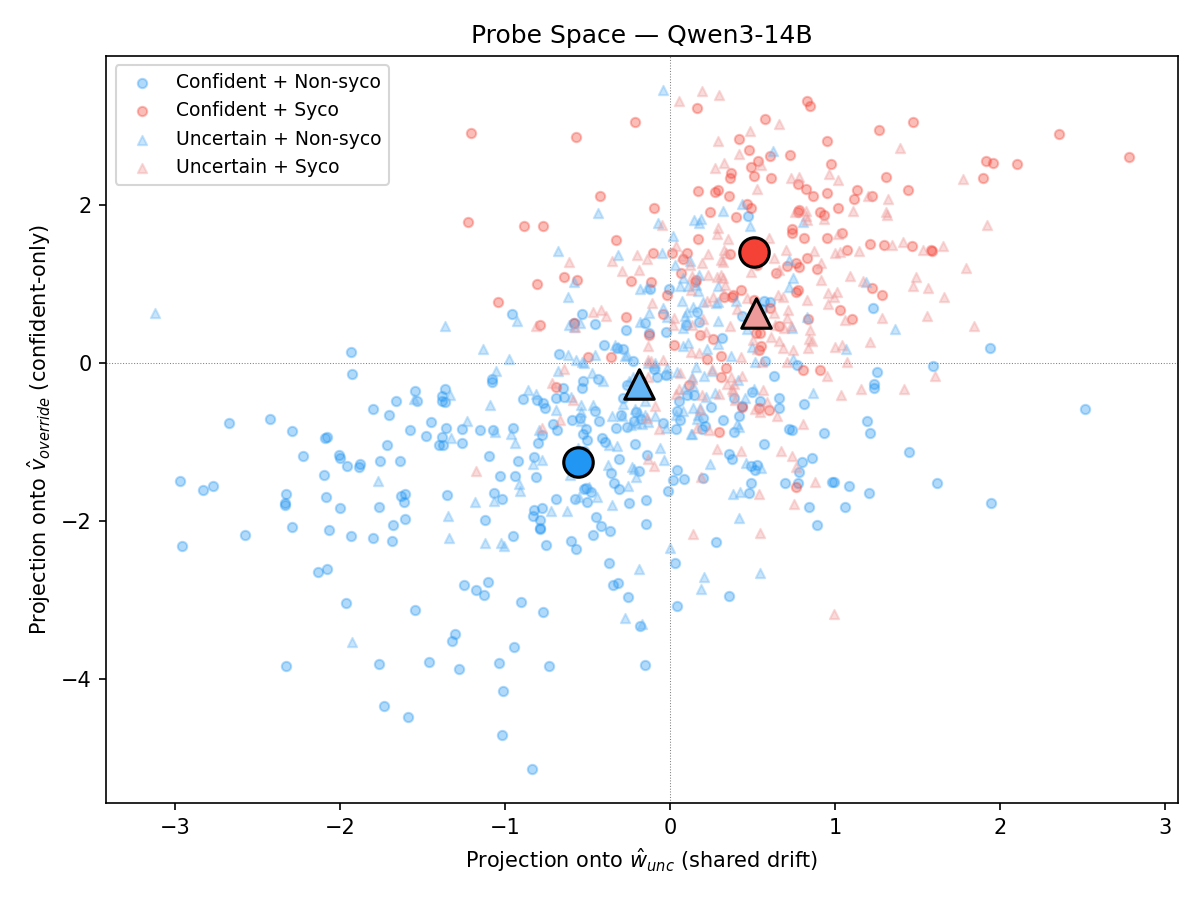
\includegraphics[width=\textwidth]{figures/geometry_probe_space.png}
\end{subfigure}
\hfill
\begin{subfigure}[t]{0.48\textwidth}
  \centering
  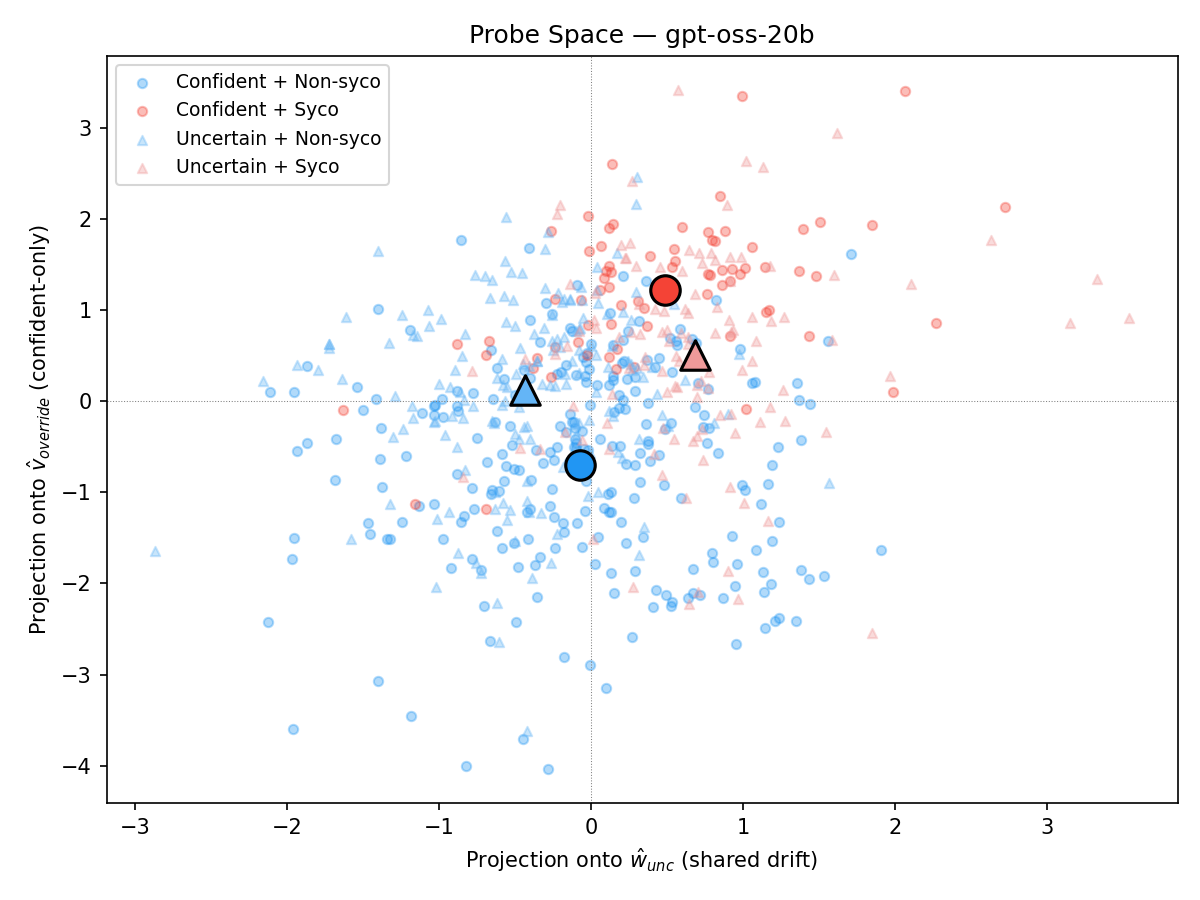
\includegraphics[width=\textwidth]{figures/geometry_probe_space_gptoss.png}
\end{subfigure}
\end{center}
\caption{Activations projected onto the $(\hat{\mathbf{w}}_{\text{unc}}, \hat{\mathbf{v}}_{\text{override}})$ basis for Qwen3-14B (left) and gpt-oss-20b (right). Large markers show group centroids. In both models, confident groups (circles) separate sharply along $\hat{\mathbf{v}}_{\text{override}}$ while uncertain groups (triangles) cluster near the origin on that axis, the signature of nested geometry.}
\label{fig:probe_space}
\end{figure*}


\subsection{MoE Routing: Standing Committees}

A natural hypothesis is that MoE routers steer confident and uncertain tokens through different experts, and that the nested geometry arises from this routing divergence.
We test this by hooking all router layers and recording expert assignments for CoT tokens across all test records.

\begin{table}[t]
\caption{MoE routing statistics (mean across all layers). Jaccard measures overlap of top dominant experts between groups.}
\label{tab:routing}
\begin{center}
\begin{small}
\begin{sc}
\begin{tabular}{lcccc}
\toprule
 & \multicolumn{2}{c}{gpt-oss-20b} & \multicolumn{2}{c}{Qwen3-MoE} \\
\cmidrule(lr){2-3}\cmidrule(lr){4-5}
Comparison & JS & Jacc. & JS & Jacc. \\
\midrule
C vs.\ U & .0007 & .94 & .0043 & .86 \\
S vs.\ NS & .0010 & .93 & .0022 & .88 \\
\bottomrule
\end{tabular}
\end{sc}
\end{small}
\end{center}
\end{table}

Table~\ref{tab:routing} shows a strong null result in both MoE models.
The router assigns the \emph{same} experts to all groups: JS divergences are three orders of magnitude below the maximum ($\ln 2 \approx 0.693$), and Jaccard overlap of dominant experts is $\geq 0.86$.
Routing entropy is effectively identical across groups ($\sim$2.73 nats in gpt-oss, $\sim$3.71 in Qwen-MoE).

We term these shared expert subsets \textbf{standing committees}: fixed MLP expert coalitions that process all inputs regardless of the model's epistemic state or behavioral outcome.
The nested geometry is computed \emph{within} these committees: the same expert parameters implement both the shared drift ($\mathbf{w}_{\text{unc}}$) and the conditional override ($\mathbf{v}_{\text{override}}$), activated by different input subspaces.
This rules out the hypothesis that sycophancy could be mitigated by modifying MoE routing decisions or fine-tuning ``sycophancy-specific'' experts (per-layer routing plots in Appendix~\ref{app:routing}).


% ============================================================================
\section{The Limits of Linear Intervention}
\label{sec:steering}

The nested geometry invites a natural intervention: subtract $\mathbf{v}_{\text{override}}$ from residual stream activations to suppress confident sycophancy, or $\mathbf{w}_{\text{overall}}$ to reduce sycophancy broadly.
We test this via activation steering on Qwen3-14B and gpt-oss-20b.

\subsection{Method}

We train three probes on the best-layer features and convert each weight vector from scaled to raw activation space via $\mathbf{w}_{\text{raw}} = \mathbf{w}_{\text{scaled}} / \boldsymbol{\sigma}_{\text{scaler}}$.
We compute $\mathbf{v}_{\text{override}} = \mathbf{w}_{\text{conf}} - \text{proj}_{\mathbf{w}_{\text{unc}}}(\mathbf{w}_{\text{conf}})$ and normalize all directions to unit norm.

During generation, we register a forward hook at the target layer that subtracts $\alpha \cdot \hat{\mathbf{d}}$ from the residual stream for steering strengths $\alpha \in \{5, 10, 20\}$.
We evaluate on all test records using greedy decoding and report sycophancy rates broken down by confidence regime.

\subsection{Null Result}

\begin{table*}[t]
\caption{Sycophancy rates (\%) under activation steering. ``Parse'' denotes the fraction of outputs where the model produced a valid answer-letter selection; unparseable outputs (incoherent or off-format text) are excluded from the sycophancy rate. Baseline rates reflect the high sycophancy of the re-prompted evaluation format. No direction achieves $> 6$ pp reduction without also collapsing parse rates.}
\label{tab:steering}
\begin{center}
\begin{small}
\begin{sc}
\begin{tabular}{lcccccc}
\toprule
 & \multicolumn{2}{c}{Qwen3-14B} & \multicolumn{2}{c}{gpt-oss-20b} & \multicolumn{2}{c}{Qwen3-30B-A3B} \\
\cmidrule(lr){2-3}\cmidrule(lr){4-5}\cmidrule(lr){6-7}
Config & All & Parse & All & Parse & All & Parse \\
\midrule
Baseline & 84.3 & 99.7 & 63.7 & 91.6 & 83.0 & 100.0 \\
\midrule
$\mathbf{w}_o$, $\alpha$=10 & 81.7 & 98.6 & 63.1 & 92.6 & 79.8 & 87.7 \\
$\mathbf{w}_o$, $\alpha$=20 & 76.2 & 97.5 & 61.3 & 91.0 & --- & 0.0 \\
$\mathbf{v}_{\text{ov}}$, $\alpha$=10 & 83.0 & 98.4 & 63.1 & 91.0 & 80.5 & 100.0 \\
$\mathbf{v}_{\text{ov}}$, $\alpha$=20 & 81.7 & 96.5 & 61.5 & 90.2 & 77.5 & 61.8 \\
Random, $\alpha$=10 & 84.0 & 98.7 & 63.1 & 92.4 & 83.4 & 100.0 \\
\bottomrule
\end{tabular}
\end{sc}
\end{small}
\end{center}
\end{table*}

Table~\ref{tab:steering} shows that no steering direction achieves meaningful sycophancy reduction without simultaneously degrading generation.
For Qwen3-14B and gpt-oss-20b, the strongest effect at $\alpha = 20$ is $\sim$3 pp (Qwen, $\mathbf{w}_{\text{overall}}$), comparable to the random control's noise floor, with parse rates declining only slightly.
Qwen3-30B-A3B exhibits the same pattern in a sharper form: at $\alpha = 20$ along $\mathbf{w}_{\text{overall}}$ the model produces zero parsable answers (parse rate $0\%$), with outputs collapsing into repetitive loops; along $\mathbf{v}_{\text{override}}$ the parse rate falls to $61.8\%$ for a $5.5$ pp drop in sycophancy. The progression---from cosmetic suppression at small $\alpha$ to outright generation collapse at large $\alpha$---is consistent with an off-manifold push rather than targeted suppression of the sycophantic feature.

\subsection{Theoretical Explanation}

We explain this null result via representational independence \citep{wollschlager2025geometry}: although $\mathbf{w}_{\text{unc}}$ and $\mathbf{v}_{\text{override}}$ are orthogonal as probe directions, subtracting one pushes activations off the data manifold into regions where subsequent layers have not been trained to operate, producing incoherent outputs rather than non-sycophantic ones.
The nested geometry is thus \emph{readable} (linear probes detect it) but not \emph{writable} via static linear intervention (causal modularity fails).

\paragraph{Implications.}
Our analysis constrains \emph{static} interventions but not dynamic ones: methods like MONICA \citep{hu2025monica} that modulate intervention strength token-by-token may succeed by keeping activations on-manifold.
Our $(\hat{\mathbf{w}}_{\text{unc}}, \hat{\mathbf{v}}_{\text{override}})$ basis provides the regime-diagnostic component such systems need.


% ============================================================================
\section{Limitations}
\label{sec:limitations}

\paragraph{Entropy and labels.}
RLHF compresses logit distributions, which may reduce measured entropy; our median split uses relative thresholds, and the quintile analysis (Table~\ref{tab:quintiles}) confirms the asymmetry scales monotonically rather than being a binary-split artifact.
Features are extracted from the intervention pass while labels are defined by control-intervention disagreement; persona-induced activation differences could partially drive the probe signal even at $K{=}0$, though nontrivial pre-generation AUROCs ($\geq 0.72$) suggest the signal reflects genuine propensity.

\paragraph{Scope.}
Our three models share RLHF/GRPO post-training; models with different routers or post-training may behave differently.
MoE routing statistics are averaged over all CoT tokens; token-local analyses could reveal subtle per-step routing differences.
Steering experiments test only single-layer, fixed-strength subtraction; geometry-aware alternatives (rotational steering, multi-layer or token-adaptive gates) remain untested.
Our probes characterize \emph{linear} geometry; nonlinear features may exist.
The dataset contains only multiple-choice opinion questions; open-ended or mathematical sycophancy \citep{petrov2025brokenmath} may differ.

\paragraph{Reproducibility.}
All experiment scripts, configurations, and analysis code are available at \url{https://anonymous.4open.science/r/sycophancy-uncertainty-E898/}. The full dataset (generated CoTs, labels, residual-stream features, and steering outputs) is released at \url{https://huggingface.co/datasets/anonymous-author-1/nested-sycophancy}.


% ============================================================================
\section{Conclusion}
\label{sec:conclusion}

Across three architectures (one dense, two MoE), we find the same nested topology: uncertain sycophancy ($\mathbf{w}_{\text{unc}}$) captures a shared component present in all sycophantic activations, while confident sycophancy adds an orthogonal truth-override ($\mathbf{v}_{\text{override}}$).
This structure is computed within fixed ``standing committees'' of MoE experts, not through differential routing, and static linear steering cannot span the orthogonal subspaces.
These findings motivate a shift to \emph{dynamic}, regime-aware intervention: the $(\hat{\mathbf{w}}_{\text{unc}}, \hat{\mathbf{v}}_{\text{override}})$ basis identifies which mechanism is active, enabling targeted, on-manifold calibration.


\bibliography{references}

%%%%%%%%%%%%%%%%%%%%%%%%%%%%%%%%%%%%%%%%%%%%%%%%%%%%%%%%%%%%%%%%%%%%%%%%%%%%%%%
% APPENDIX
%%%%%%%%%%%%%%%%%%%%%%%%%%%%%%%%%%%%%%%%%%%%%%%%%%%%%%%%%%%%%%%%%%%%%%%%%%%%%%%
\appendix
\onecolumn

\section{Full Probe Results}
\label{app:probes}

Tables~\ref{tab:app_probes_qwen}--\ref{tab:app_probes_qwenmoe} report test AUROC for all layer $\times$ CoT depth configurations.

\begin{table}[H]
\caption{Test AUROC across all layer $\times$ K configurations for Qwen3-14B.}
\label{tab:app_probes_qwen}
\begin{center}
\begin{small}
\begin{sc}
\begin{tabular}{lcccccc}
\toprule
Layer & $K$0 & $K$10 & $K$25 & $K$50 & $K$75 & $K$100 \\
\midrule
L10 & .699 & .742 & .773 & .827 & .850 & .872 \\
L20 & .782 & .844 & .855 & .877 & .891 & .904 \\
L30 & \textbf{.790} & .822 & .851 & .884 & .898 & \textbf{.909} \\
L35 & .788 & .813 & .839 & .880 & .886 & .902 \\
\bottomrule
\end{tabular}
\end{sc}
\end{small}
\end{center}
\end{table}

\begin{table}[H]
\caption{Test AUROC across all layer $\times$ K configurations for gpt-oss-20b.}
\label{tab:app_probes_gptoss}
\begin{center}
\begin{small}
\begin{sc}
\begin{tabular}{lcccccc}
\toprule
Layer & $K$0 & $K$10 & $K$25 & $K$50 & $K$75 & $K$100 \\
\midrule
L6  & .772 & .767 & .767 & .821 & .848 & .864 \\
L12 & .776 & .805 & .820 & .857 & .872 & \textbf{.909} \\
L18 & \textbf{.810} & .811 & .836 & .843 & .867 & .908 \\
L21 & .795 & .796 & .812 & .836 & .857 & .896 \\
\bottomrule
\end{tabular}
\end{sc}
\end{small}
\end{center}
\end{table}

\begin{table}[H]
\caption{Test AUROC across all layer $\times$ K configurations for Qwen3-30B-A3B.}
\label{tab:app_probes_qwenmoe}
\begin{center}
\begin{small}
\begin{sc}
\begin{tabular}{lcccccc}
\toprule
Layer & $K$0 & $K$10 & $K$25 & $K$50 & $K$75 & $K$100 \\
\midrule
L12 & .679 & .714 & .740 & .770 & .761 & .769 \\
L24 & .714 & .756 & .793 & .791 & .799 & .823 \\
L36 & \textbf{.720} & .757 & .784 & .792 & .812 & \textbf{.827} \\
L42 & .715 & .745 & .765 & .781 & .802 & .825 \\
\bottomrule
\end{tabular}
\end{sc}
\end{small}
\end{center}
\end{table}


\section{AUROC by Entropy Quintile (Extended)}
\label{app:quintiles}

\begin{table}[H]
\caption{AUROC by entropy quintile for Qwen3-14B (L30 K100).}
\label{tab:app_quintiles_qwen}
\begin{center}
\begin{small}
\begin{sc}
\begin{tabular}{lccccc}
\toprule
 & Q1 & Q2 & Q3 & Q4 & Q5 \\
\midrule
$n$ (pos rate) & 154 (31.8\%) & 154 (34.4\%) & 154 (39.6\%) & 154 (49.4\%) & 154 (54.6\%) \\
AUROC & \textbf{.998} & .949 & .890 & .854 & .755 \\
\bottomrule
\end{tabular}
\end{sc}
\end{small}
\end{center}
\end{table}

\begin{table}[H]
\caption{AUROC by entropy quintile for gpt-oss-20b (L12 K100).}
\label{tab:app_quintiles_gptoss}
\begin{center}
\begin{small}
\begin{sc}
\begin{tabular}{lccccc}
\toprule
 & Q1 & Q2 & Q3 & Q4 & Q5 \\
\midrule
$n$ (pos rate) & 124 (15.3\%) & 124 (21.8\%) & 124 (32.3\%) & 124 (25.8\%) & 124 (59.7\%) \\
AUROC & .901 & .918 & .922 & .868 & .890 \\
\bottomrule
\end{tabular}
\end{sc}
\end{small}
\end{center}
\end{table}

\begin{table}[H]
\caption{AUROC by entropy quintile for Qwen3-30B-A3B (L36 K100).}
\label{tab:app_quintiles_qwenmoe}
\begin{center}
\begin{small}
\begin{sc}
\begin{tabular}{lccccc}
\toprule
 & Q1 & Q2 & Q3 & Q4 & Q5 \\
\midrule
$n$ (pos rate) & 150 (22.7\%) & 150 (32.0\%) & 150 (43.3\%) & 150 (48.7\%) & 149 (49.7\%) \\
AUROC & .956 & .933 & .769 & .744 & .657 \\
\bottomrule
\end{tabular}
\end{sc}
\end{small}
\end{center}
\end{table}


\section{Geometric Analysis Details}
\label{app:geometry}

\begin{table}[H]
\caption{Full geometric statistics across all three models.}
\label{tab:app_geometry}
\begin{center}
\begin{small}
\begin{tabular}{lccc}
\toprule
Statistic & Qwen3-14B & gpt-oss-20b & Qwen3-MoE \\
\midrule
$\cos(\mathbf{w}_{\text{conf}}, \mathbf{w}_{\text{unc}})$ & 0.057 & 0.084 & 0.102 \\
$\cos(\mathbf{w}_{\text{conf}}, \mathbf{w}_{\text{overall}})$ & 0.441 & 0.504 & 0.449 \\
$\cos(\mathbf{w}_{\text{unc}}, \mathbf{w}_{\text{overall}})$ & 0.742 & 0.702 & 0.714 \\
Decomposition $\alpha$ & 0.034 & 0.059 & 0.063 \\
$\|\mathbf{w}_{\text{conf}}\|$ & 6.28 & 6.66 & 8.94 \\
$\|\mathbf{w}_{\text{unc}}\|$ & 10.60 & 9.45 & 14.44 \\
$\|\alpha\mathbf{w}_{\text{unc}}\|$ & 0.36 & 0.56 & 0.91 \\
$\|\mathbf{v}_{\text{override}}\|$ & 6.27 & 6.64 & 8.89 \\
Fraction explained & 0.33\% & 0.71\% & 1.05\% \\
PCA var.\ (PC1, PC2) & 14.5\%, 11.4\% & 13.3\%, 12.1\% & 14.4\%, 10.8\% \\
\bottomrule
\end{tabular}
\end{small}
\end{center}
\end{table}


\section{PCA Visualizations}
\label{app:pca}

\begin{figure}[H]
\begin{center}
\begin{subfigure}[t]{0.48\textwidth}
  \centering
  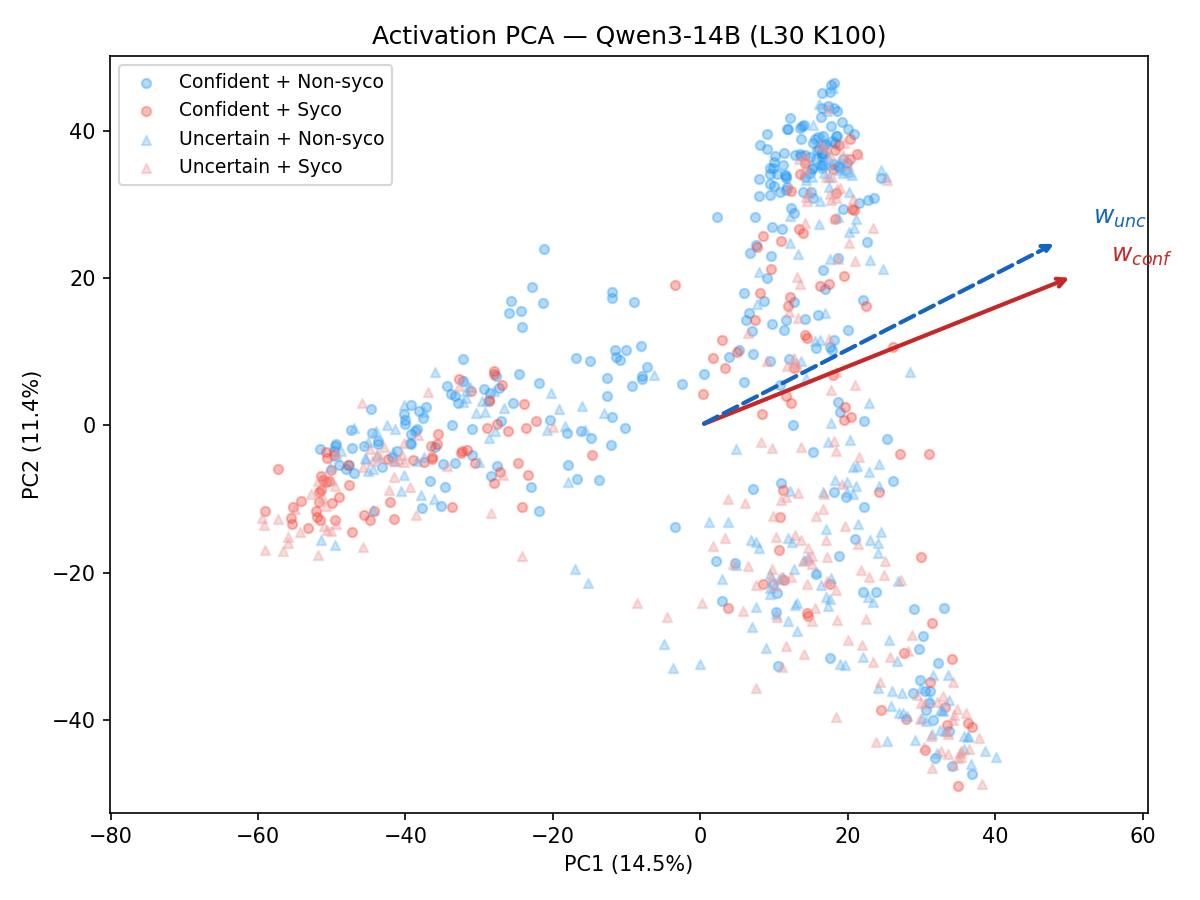
\includegraphics[width=\textwidth]{figures/geometry_pca.png}
  \caption{Qwen3-14B (L30, K100)}
\end{subfigure}
\hfill
\begin{subfigure}[t]{0.48\textwidth}
  \centering
  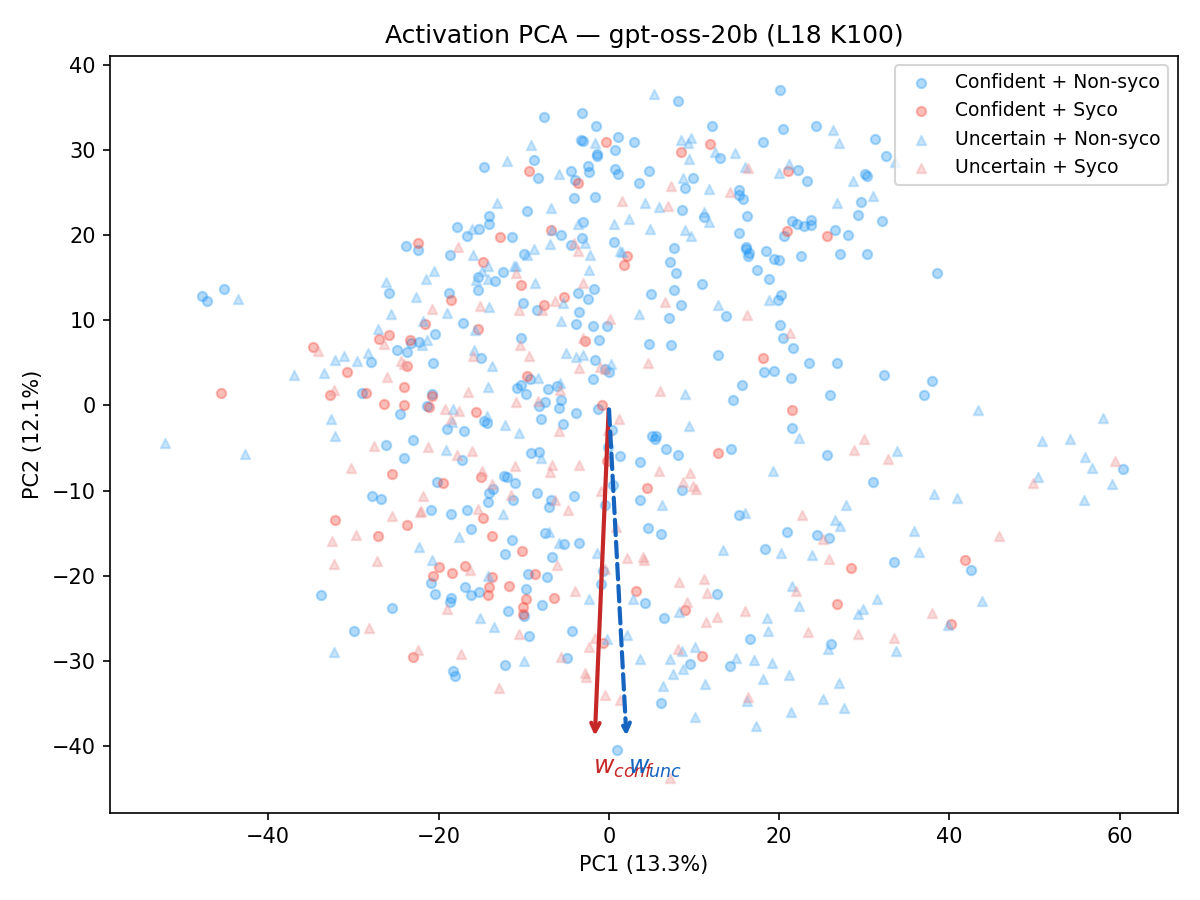
\includegraphics[width=\textwidth]{figures/geometry_pca_gptoss.png}
  \caption{gpt-oss-20b (L18, K100)}
\end{subfigure}
\end{center}
\caption{PCA of residual stream activations colored by group. Probe directions $\mathbf{w}_{\text{unc}}$ and $\mathbf{w}_{\text{conf}}$ are overlaid.}
\label{fig:pca}
\end{figure}


\section{MoE Routing Analysis}
\label{app:routing}

\begin{figure}[H]
\begin{center}
\begin{subfigure}[t]{0.48\textwidth}
  \centering
  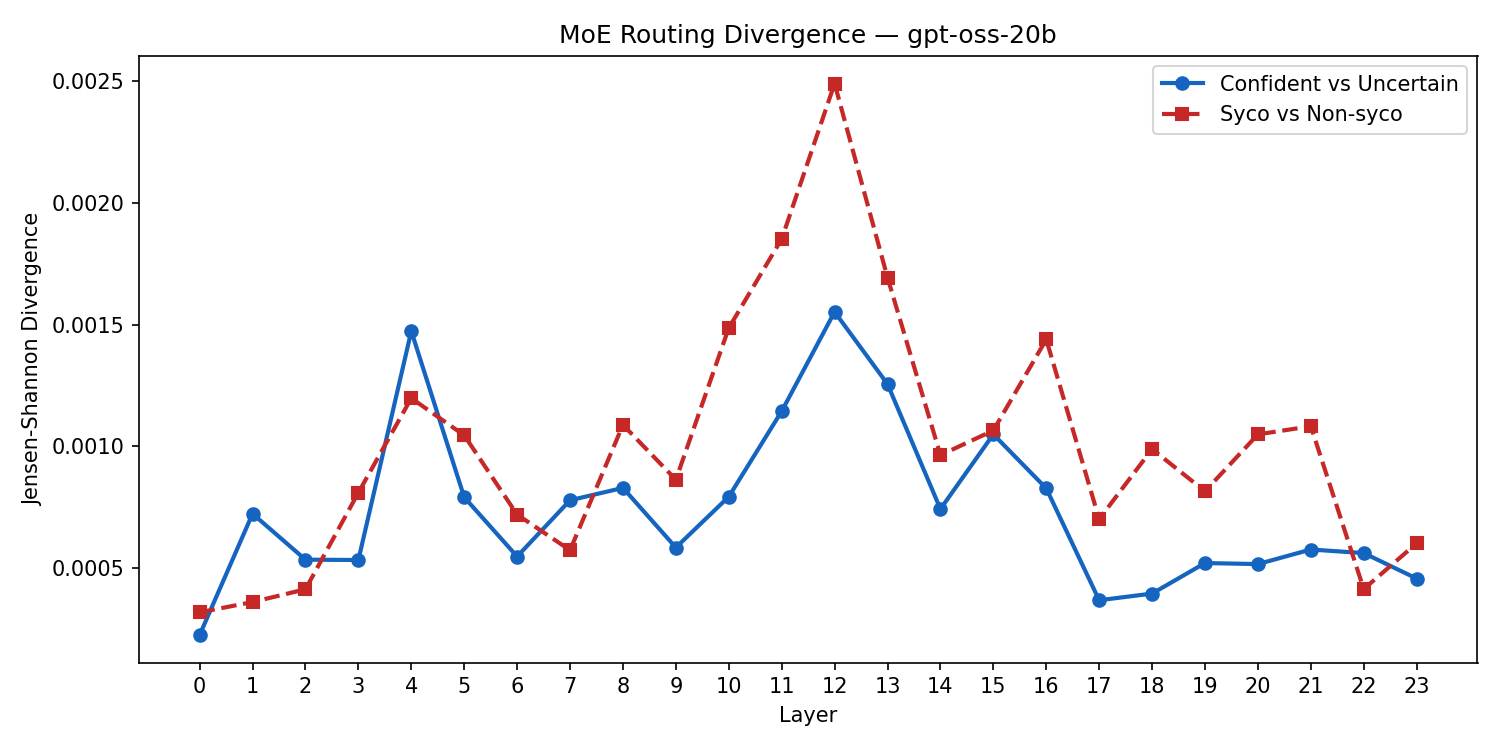
\includegraphics[width=\textwidth]{figures/moe_routing_divergence.png}
  \caption{gpt-oss-20b: JS divergence per layer}
\end{subfigure}
\hfill
\begin{subfigure}[t]{0.48\textwidth}
  \centering
  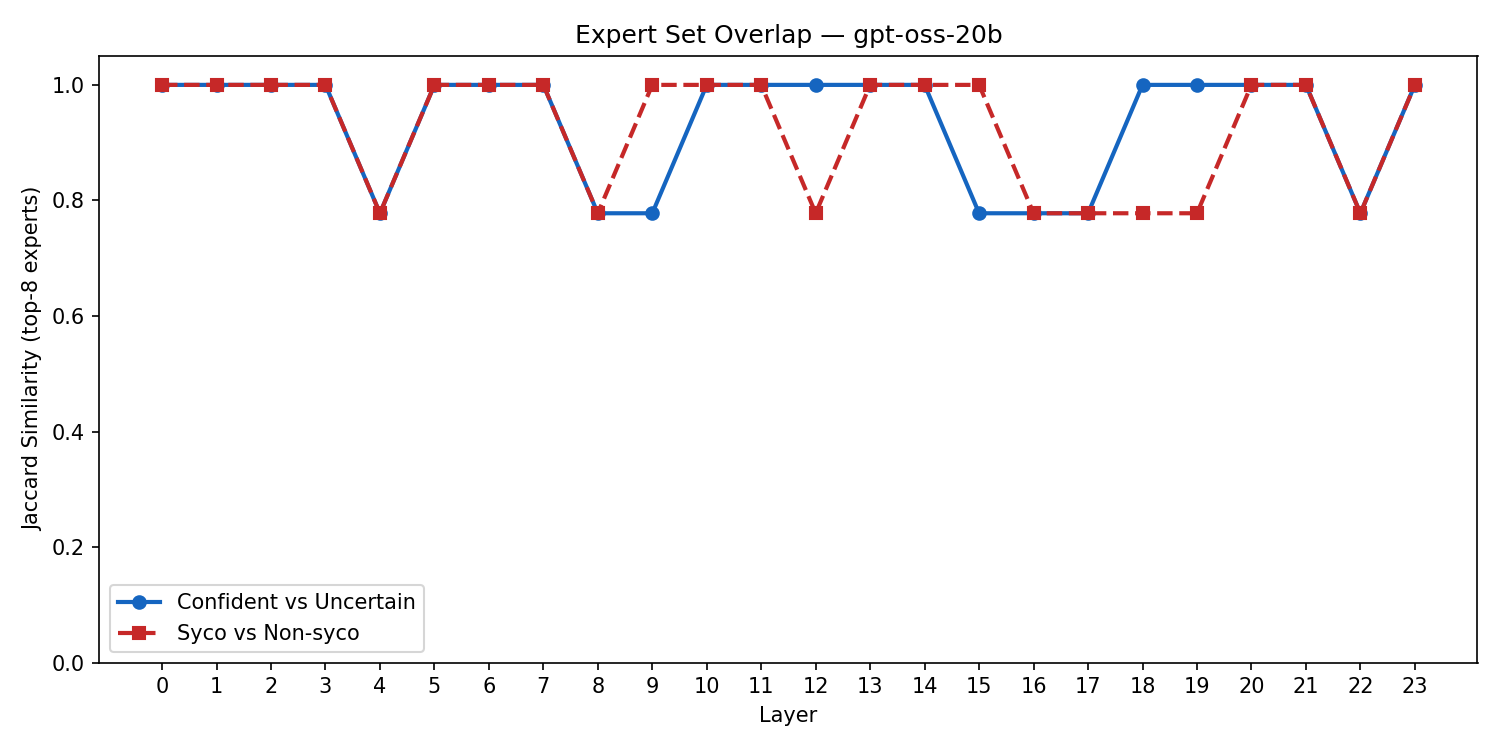
\includegraphics[width=\textwidth]{figures/moe_routing_jaccard.png}
  \caption{gpt-oss-20b: Jaccard similarity per layer}
\end{subfigure}
\end{center}
\caption{MoE routing statistics across all 24 layers of gpt-oss-20b. JS divergence remains $< 0.003$ for all layers, and Jaccard overlap $\geq 0.75$ per layer (mean 0.93), confirming the standing committee hypothesis.}
\label{fig:routing}
\end{figure}


\section{Projection Group Statistics}
\label{app:projections}

\begin{table}[H]
\caption{Mean projection ($\pm$ SE) onto each axis by group. C = confident, U = uncertain, NS = non-sycophantic, S = sycophantic.}
\label{tab:app_projections}
\begin{center}
\begin{small}
\begin{tabular}{lcccc}
\toprule
 & \multicolumn{2}{c}{$\hat{\mathbf{w}}_{\text{unc}}$} & \multicolumn{2}{c}{$\hat{\mathbf{v}}_{\text{override}}$} \\
\cmidrule(lr){2-3}\cmidrule(lr){4-5}
Group & Mean & SE & Mean & SE \\
\midrule
\multicolumn{5}{c}{\emph{Qwen3-14B}} \\
C+NS ($n$=259) & $-$0.557 & 0.063 & $-$1.247 & 0.070 \\
C+S ($n$=133)  & +0.509 & 0.060 & +1.406 & 0.087 \\
U+NS ($n$=188) & $-$0.186 & 0.044 & $-$0.261 & 0.086 \\
U+S ($n$=190)  & +0.521 & 0.041 & +0.642 & 0.083 \\
\midrule
\multicolumn{5}{c}{\emph{gpt-oss-20b}} \\
C+NS ($n$=258) & $-$0.068 & 0.051 & $-$0.701 & 0.068 \\
C+S ($n$=74)   & +0.488 & 0.091 & +1.215 & 0.091 \\
U+NS ($n$=170) & $-$0.431 & 0.048 & +0.118 & 0.076 \\
U+S ($n$=118)  & +0.688 & 0.065 & +0.502 & 0.101 \\
\midrule
\multicolumn{5}{c}{\emph{Qwen3-30B-A3B}} \\
C+NS ($n$=264) & $-$0.396 & 0.052 & $-$0.846 & 0.062 \\
C+S ($n$=115)  & +0.298 & 0.042 & +0.765 & 0.055 \\
U+NS ($n$=191) & +0.014 & 0.030 & +0.177 & 0.052 \\
U+S ($n$=179)  & +0.298 & 0.034 & +0.451 & 0.052 \\
\bottomrule
\end{tabular}
\end{small}
\end{center}
\end{table}


\section{Subspace Inclusion Analysis}
\label{app:subspace}

To further validate the nested geometry claim, we apply standard subspace comparison methods to the discriminant subspaces of confident and uncertain sycophancy.
We build $k$-dimensional discriminant subspaces for each regime using the between-class mean difference (Fisher direction) plus the top within-class scatter components, and evaluate asymmetric inclusion, projection residuals, and principal angles.
All computations use precomputed features at the best layer for each model.

\paragraph{Asymmetric subspace inclusion.}
If unc$\subset$conf, a low-dimensional uncertain subspace ($k_{\text{sub}}$) should be well-captured by a higher-dimensional confident subspace ($k_{\text{super}}$), but not vice versa.
Table~\ref{tab:app_subspace} confirms this: inclusion(unc$\subset$conf) consistently exceeds inclusion(conf$\subset$unc) for Qwen3-14B and Qwen3-30B-A3B (permutation $p < 0.001$).
The effect is weaker for gpt-oss-20b ($p = 0.096$), consistent with its smaller cross-prediction asymmetry.

\paragraph{Probe direction angle.}
The probe weight vectors $\mathbf{w}_{\text{conf}}$ and $\mathbf{w}_{\text{unc}}$ are nearly orthogonal in all models ($84$--$86^{\circ}$), consistent with the cosine similarities reported in Table~\ref{tab:geometry}.

\paragraph{Projection residuals.}
When projecting the uncertain discriminant subspace onto the confident one, less information is lost (lower residual) than in the reverse direction, providing complementary evidence for the nesting.

\begin{table}[H]
\caption{Subspace analysis across all three models ($k_{\text{sub}}=5$, $k_{\text{super}}=20$).}
\label{tab:app_subspace}
\begin{center}
\begin{small}
\begin{tabular}{lccc}
\toprule
& \textbf{Qwen3-14B} & \textbf{gpt-oss-20b} & \textbf{Qwen3-30B} \\
\midrule
\multicolumn{4}{l}{\textit{Subspace inclusion}} \\
\quad inc(unc$\subset$conf) & 0.780 & 0.821 & 0.808 \\
\quad inc(conf$\subset$unc) & 0.668 & 0.813 & 0.651 \\
\quad $\Delta$ (asymmetry) & +0.112 & +0.008 & +0.157 \\
\quad perm.\ $p$-value & $<$0.001 & 0.096 & $<$0.001 \\
\midrule
\multicolumn{4}{l}{\textit{Projection residual ($k_{\text{from}}=5, k_{\text{onto}}=20$)}} \\
\quad resid(unc$\to$conf) & 0.160 & 0.127 & 0.112 \\
\quad resid(conf$\to$unc) & 0.206 & 0.141 & 0.186 \\
\quad $\Delta$ & +0.046 & +0.014 & +0.074 \\
\midrule
\multicolumn{4}{l}{\textit{Geometry}} \\
\quad Probe angle ($^\circ$) & 86.2 & 84.6 & 84.1 \\
\quad Linear CKA & 0.052 & 0.047 & 0.050 \\
\quad Principal angles ($k$=5, mean) & 43.8$^\circ$ & 42.7$^\circ$ & 42.1$^\circ$ \\
\bottomrule
\end{tabular}
\end{small}
\end{center}
\end{table}


\end{document}
